% Generated by eval/realworld/scripts/12-charts.py. Do not edit.
\subsection{Broader comparison}
\label{sec:realworld-broad}
\emergencystretch=8em

The record-system matrix in Table~\ref{tab:rw-matrix} is unchanged. This subsection adds the detector, citation, gateway, and hosted-model measurements from the same machine.

Lattice's OpenAI-compatible adapter called \path{https://openrouter.ai/api/v1}. The catalog check found 8 of the requested \texttt{:free} ids, and the listed prompt and completion prices were 0. Completed model rows: 8. Upstream HTTP 429 responses were retried. Pacing sleeps, that backoff, and the HTTP time of a failed attempt are excluded from Lattice time and from the end-to-end denominator. Provider time includes waiting for the response headers and reading the body. An earlier subtraction stopped at the headers, so the body download was counted as Lattice time. Completion tokens are capped at the value recorded in \texttt{openrouter.json} (8192 in this run). Models whose catalog lists a reasoning parameter also receive \texttt{reasoning.effort=low}. A 400 that rejects that field is retried once without it. Temperature is injected by the fetch wrapper. Table~\ref{tab:rw-models} uses the provider string returned on the chat response. A drift cell is distinct successful answers, successful calls, and attempts. Replay uses only calls that returned. The local row is the earlier Ollama run (drift n=3, overhead n=5). Hosted drift used n=10 when the call returned.
 On the local Ollama run, the median time outside the HTTP call was 2.4~ms (p95 15.0~ms, 0.439\% of that run's signed wall time). That localhost call returns the body with the headers, so the gap is processing time. Across hosted models with a successful signed short prompt, the median Lattice processing time was 1.10--1.69~ms. Table~\ref{tab:rw-lattice} gives the median and p95 in milliseconds and as a percentage of end-to-end time. The packed Lattice prompt added 61--83 prompt tokens at the median versus the one-line direct prompt. The paired provider-time difference on that longer prompt had medians from -2398 to 3352~ms. A negative value means the packed call returned sooner. The difference changes sign and is often larger than a short extra prefill can explain, because completion length, including reasoning tokens, moves the provider time by seconds. It is reported separately and is not added to Lattice processing time.

\begin{table*}[t]
\centering
\caption{Short-prompt latency and the RAG, replay, ticket, and crew checks. Lattice ms is the median signed processing time, excluding provider time, retries, and backoff. Drift cells are unique successes / successes / attempts. Replay is restricted to calls that returned a receipt. Receipt columns are the single-agent return and the crew return.}
\label{tab:rw-models}
\footnotesize
\resizebox{\textwidth}{!}{%
\begin{tabular}{@{}l l r r r r r l r l r r@{}}
\toprule
Model & Provider & Plain ms & Signed ms & Lattice ms & Drift 0 & Drift 0.7 & Cited & Replay & Ticket leak & Agent rcpt & Crew rcpt \\
\midrule
llama3.2:3b local & Ollama & 278 & 559 & 2.45 & 1/3/3 & 1/3/3 & 3/3, 3/3 & 6/6 & no & 0 & 4 \\
\texttt{minimax/minimax-m3.1-flash:free} & Minimax & 3677 & 1489 & 1.69 & 3/10/10 & 1/10/10 & 10/10, 10/10 & 20/20 & no & 0 & 4 \\
\texttt{xingchen-agi/xing4.0-29b-a4b:free} & Phala & 3124 & 9820 & 1.21 & 4/8/10 & 3/3/10 & 8/8, 3/3 & 11/11 & no & 0 & 3 \\
\texttt{nvidia/nemotron-3.5-super-vl:free} & Nvidia & 675 & 845 & 1.20 & 1/10/10 & 2/10/10 & 10/10, 10/10 & 20/20 & no & 0 & 4 \\
\texttt{nvidia/nemotron-3.5-lightning:free} & Nvidia & 1319 & 2701 & 1.10 & 4/10/10 & 6/10/10 & 10/10, 10/10 & 20/20 & no & 0 & 3 \\
\texttt{dots-studio/dots-3-note-preview:free} & AtlasCloud & 1145 & 1275 & 1.50 & 2/10/10 & 3/10/10 & 10/10, 10/10 & 20/20 & no & 0 & 4 \\
\texttt{liquid/lfm-2.5-2.6b:free} & Liquid & 4179 & 4649 & 1.65 & 3/10/10 & 2/10/10 & 10/10, 10/10 & 20/20 & no & fail & fail \\
\texttt{thinkingmachines/inkling-small:free} & --- & --- & --- & --- & --- & --- & ---, --- & --- & --- & --- & --- \\
\texttt{poolside/laguna-s-2.1:free} & Poolside & 715 & 1413 & 1.56 & 1/10/10 & 4/10/10 & 10/10, 10/10 & 20/20 & no & 0 & 4 \\
\bottomrule
\end{tabular}}
\end{table*}

\begin{table*}[t]
\centering
\caption{Pure Lattice processing on the signed short prompt. The percentage uses end-to-end time with backoff removed. Extra tokens are Lattice prompt tokens minus the direct prompt tokens. Provider delta is the signed provider time minus the direct provider time, in milliseconds, and is the latency of the longer packed prompt.}
\label{tab:rw-lattice}
\footnotesize
\resizebox{\textwidth}{!}{%
\begin{tabular}{@{}l r r r r r r@{}}
\toprule
Model & ms p50 & ms p95 & \% p50 & \% p95 & Extra tokens & Provider delta \\
\midrule
llama3.2:3b local & 2.45 & 14.96 & 0.439 & 2.469 & --- & --- \\
\texttt{minimax/minimax-m3.1-flash:free} & 1.69 & 3.66 & 0.218 & 0.327 & 63 & -2398 \\
\texttt{xingchen-agi/xing4.0-29b-a4b:free} & 1.21 & 3.50 & 0.019 & 0.019 & 83 & 3352 \\
\texttt{nvidia/nemotron-3.5-super-vl:free} & 1.20 & 2.03 & 0.138 & 0.260 & 80 & 169 \\
\texttt{nvidia/nemotron-3.5-lightning:free} & 1.10 & 1.96 & 0.053 & 0.082 & 82 & 1703 \\
\texttt{dots-studio/dots-3-note-preview:free} & 1.50 & 1.90 & 0.123 & 0.141 & 74 & 59 \\
\texttt{liquid/lfm-2.5-2.6b:free} & 1.65 & 4.09 & 0.035 & 0.076 & 61 & 1005 \\
\texttt{thinkingmachines/inkling-small:free} & --- & --- & --- & --- & --- & --- \\
\texttt{poolside/laguna-s-2.1:free} & 1.56 & 4.01 & 0.142 & 0.266 & 76 & 318 \\
\bottomrule
\end{tabular}}
\end{table*}

\path{thinkingmachines/inkling-small:free} is in the public catalog at price 0. Every measured call was rejected with HTTP 403 and the message that the model is only available on agentic harnesses, so this row has no latency sample.
\path{liquid/lfm-2.5-2.6b:free} returned HTTP 504 on the single-agent call (Provider returned error). That call is a provider failure, not a receipt or citation result.
\path{liquid/lfm-2.5-2.6b:free} returned HTTP 504 on the crew call (Provider returned error). That call is a provider failure, not a receipt or citation result.

On a 16$\times$16 solid red PNG, \path{nvidia/nemotron-3.5-super-vl:free} answered red from a direct \texttt{image\_url} part: yes (answer red). The Lattice image artifact answered red: no (answer blue). The PNG bytes were present in the Lattice request body: yes. The direct response provider was Nvidia. This vision call set \texttt{reasoning.effort=none}.
The text arms use reasoning.effort=low. On this vision call, effort low and effort minimal each spent 8192 completion tokens on reasoning and returned empty content. This recorded call sets reasoning.effort=none. Lattice inlines the PNG in the text JSON. The direct arm sends an image\_url part.

Document-level precision, recall, and F1 use the harness overlap rule: a document is a true positive when any predicted span of that type overlaps a gold span. An undefined F1 means there were no positive predictions, or no gold documents and no false positives. spaCy \texttt{en\_core\_web\_sm} emits none of the four labels, so its precision and F1 are undefined and its recall is zero wherever a gold span exists. Figure~\ref{fig:rw-pii-f1} omits those undefined bars.

\begin{table*}[t]
\centering
\caption{ai4privacy English validation, document level. Latency is the median milliseconds per document.}
\label{tab:rw-pii-ai4}
\footnotesize
\resizebox{\textwidth}{!}{%
\begin{tabular}{@{}l rrr rrr rrr rrr r@{}}
\toprule
Tool & \multicolumn{3}{c}{Email} & \multicolumn{3}{c}{US SSN} & \multicolumn{3}{c}{US phone} & \multicolumn{3}{c}{Card} & ms \\
& P & R & F1 & P & R & F1 & P & R & F1 & P & R & F1 & \\
\midrule
Lattice & 0.955 & 0.979 & 0.967 & 0.325 & 0.436 & 0.372 & 0.316 & 0.333 & 0.324 & 0.000 & --- & --- & 0.007 \\
presidio & 0.974 & 0.999 & 0.986 & 0.334 & 0.502 & 0.401 & 0.295 & 0.504 & 0.372 & 0.000 & --- & --- & 9.413 \\
spaCy sm & --- & 0.000 & --- & --- & 0.000 & --- & --- & 0.000 & --- & --- & --- & --- & 8.199 \\
gliner-small & 0.695 & 0.625 & 0.658 & 0.283 & 0.458 & 0.350 & 0.228 & 0.161 & 0.189 & 0.000 & --- & --- & 52.862 \\
llm-guard-anonymize & 0.965 & 0.999 & 0.982 & 0.991 & 0.450 & 0.619 & 0.650 & 0.962 & 0.776 & 0.000 & --- & --- & 142.115 \\
\bottomrule
\end{tabular}}
\end{table*}

\begin{table*}[t]
\centering
\caption{Gretel English finance test, same document-level rule. Gold credit-card spans in this file use the label \texttt{credit\_card\_number}.}
\label{tab:rw-pii-gretel}
\footnotesize
\resizebox{\textwidth}{!}{%
\begin{tabular}{@{}l rrr rrr rrr rrr r@{}}
\toprule
Tool & \multicolumn{3}{c}{Email} & \multicolumn{3}{c}{US SSN} & \multicolumn{3}{c}{US phone} & \multicolumn{3}{c}{Card} & ms \\
& P & R & F1 & P & R & F1 & P & R & F1 & P & R & F1 & \\
\midrule
Lattice & 0.522 & 0.934 & 0.670 & 0.161 & 0.771 & 0.266 & 0.521 & 0.702 & 0.598 & 0.881 & 0.500 & 0.638 & 0.020 \\
presidio & 0.526 & 0.934 & 0.673 & 0.244 & 0.729 & 0.366 & 0.458 & 0.786 & 0.579 & 0.833 & 0.405 & 0.545 & 25.627 \\
spaCy sm & --- & 0.000 & --- & --- & 0.000 & --- & --- & 0.000 & --- & --- & 0.000 & --- & 21.623 \\
gliner-small & 0.237 & 0.511 & 0.324 & 0.090 & 0.557 & 0.155 & 0.338 & 0.234 & 0.277 & 0.165 & 0.500 & 0.248 & 156.490 \\
llm-guard-anonymize & 0.528 & 0.952 & 0.679 & 0.984 & 0.857 & 0.916 & 0.757 & 0.952 & 0.843 & 0.361 & 0.581 & 0.446 & 426.513 \\
\bottomrule
\end{tabular}}
\end{table*}

presidio: Pattern and spaCy recognizers for the four in-scope Presidio entities.
spacy-en\_core\_web\_sm: Default NER labels. None of PERSON, ORG, GPE, DATE, or CARDINAL are mapped onto email, US SSN, US phone, or credit card.
GLiNER's processor truncated documents longer than 384 tokens during this scoring run.
llm-guard-anonymize: Default Anonymize scanner with a fresh Vault in each batch process. The DeBERTa checkpoint is finetuned on ai4privacy, so the English validation score can be optimistic. A single process was OOM-killed on long inputs, so each document is analyzed in 1500-character windows with 200 characters of overlap and the scanner process exits every 250 documents. Raw SSN labels are mapped when the NER map returns them unchanged.
guardrails-detect-pii is from docs, not measured: ImportError: cannot import name 'DetectPII' from 'guardrails.hub'
nemo-guardrails is from docs, not measured: nemoguardrails is not installed, and en\_core\_web\_lg is not downloaded. The built-in sensitive-data rails call Presidio, which is scored on its own. The library also documents a separate GLiNER rail.

\begin{figure}[t]
\centering
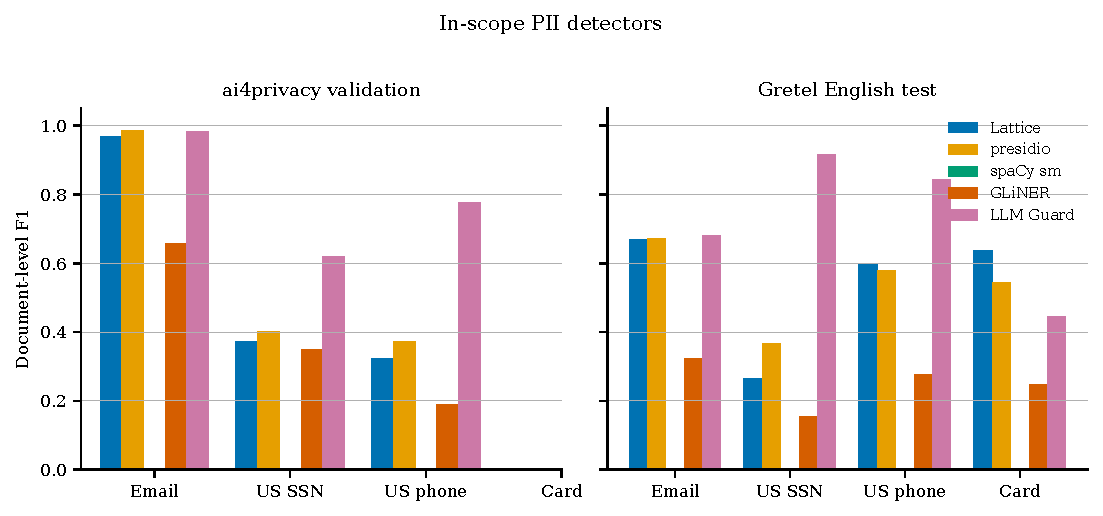
\includegraphics[width=\linewidth]{rw-pii-f1.pdf}
\caption{Document-level F1. A missing bar is an undefined F1.}
\label{fig:rw-pii-f1}
\end{figure}

\begin{figure}[t]
\centering
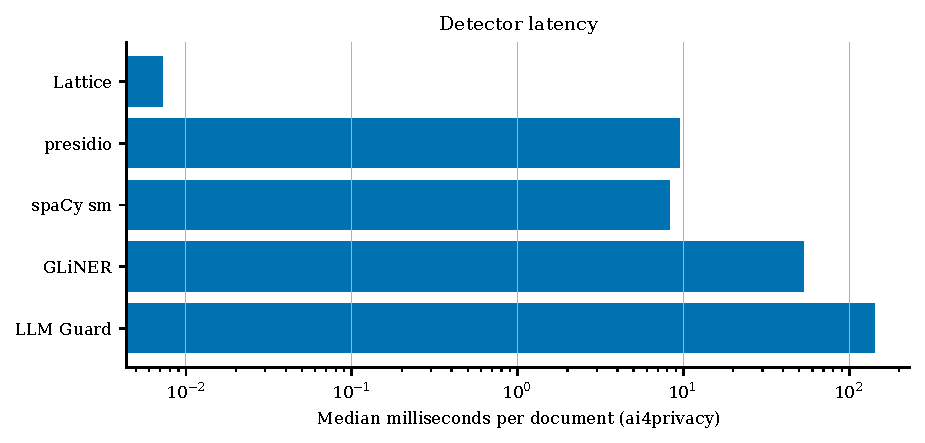
\includegraphics[width=0.86\linewidth]{rw-pii-latency.pdf}
\caption{Median detector time per ai4privacy document. The axis is logarithmic.}
\label{fig:rw-pii-latency}
\end{figure}

On ASQA dev (n=948), a case-sensitive Wikipedia title substring matches 525 long answers and a case-insensitive substring matches 605. Square-bracket citations appear in 2 answers and overlap a gold title in 0. \texttt{mustCite} accepts a gold title in 7. These three checks are different predicates.
 A local cross-encoder, \path{typeform/distilbert-base-uncased-mnli}, scored 696 of 948 pairs and labeled 296 entailed (empty 252, NEUTRAL 211, CONTRADICTION 189, ENTAILMENT 296). Median classification time was 820.0~ms. The premise is the gold knowledge text truncated to 1,800 characters and the hypothesis is the long answer. Pairs with an empty premise or answer were not scored. This is a support label, not a citation-string check.

\begin{figure}[t]
\centering
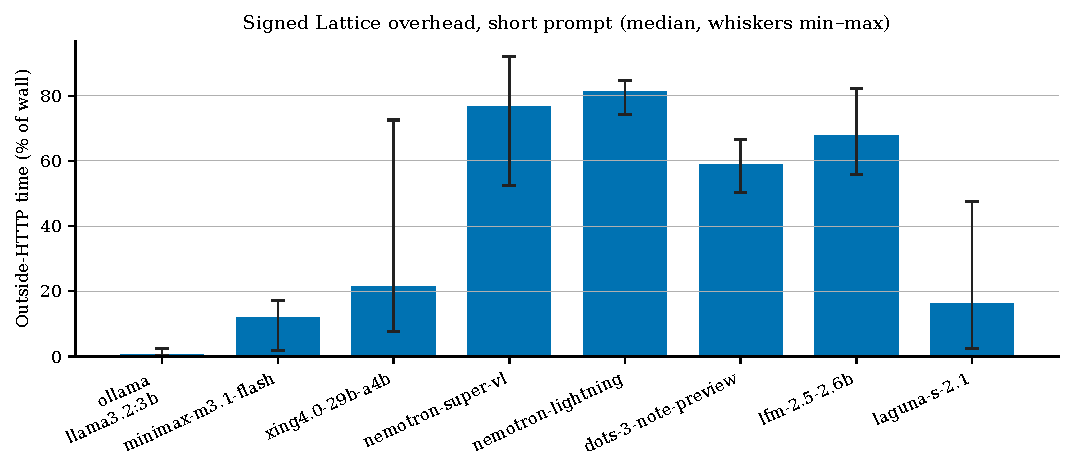
\includegraphics[width=\linewidth]{rw-overhead-pct.pdf}
\caption{Signed Lattice processing time as a percentage of end-to-end time. End-to-end time is Lattice processing plus provider time plus failed-attempt HTTP time. Backoff is excluded. The bar is the median and the whiskers run from the minimum to the maximum. The local bar is wall time minus the localhost HTTP call from the earlier Ollama run.}
\label{fig:rw-overhead-pct}
\end{figure}

\begin{figure}[t]
\centering
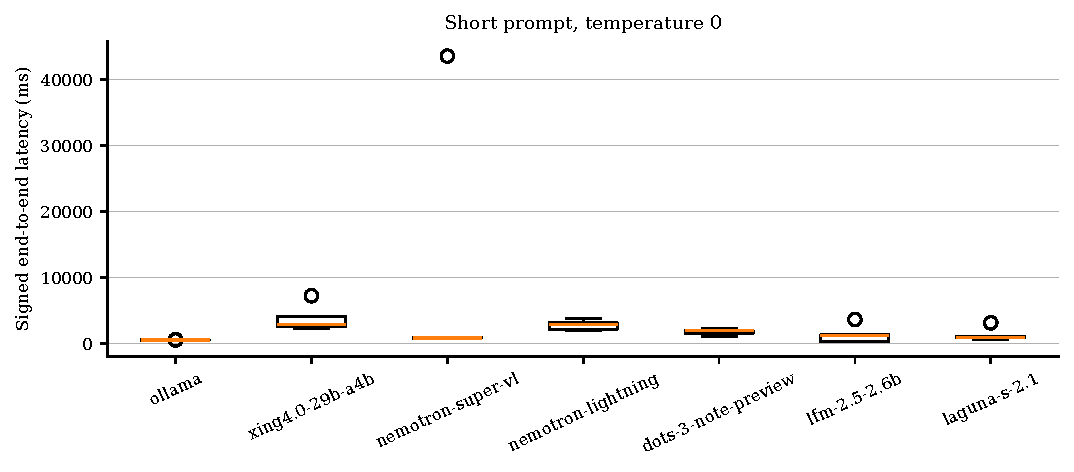
\includegraphics[width=\linewidth]{rw-latency-dist.pdf}
\caption{Signed short-prompt latency. Ollama is five trials. Each hosted row is the successful signed trials.}
\label{fig:rw-latency-dist}
\end{figure}

\begin{figure}[t]
\centering
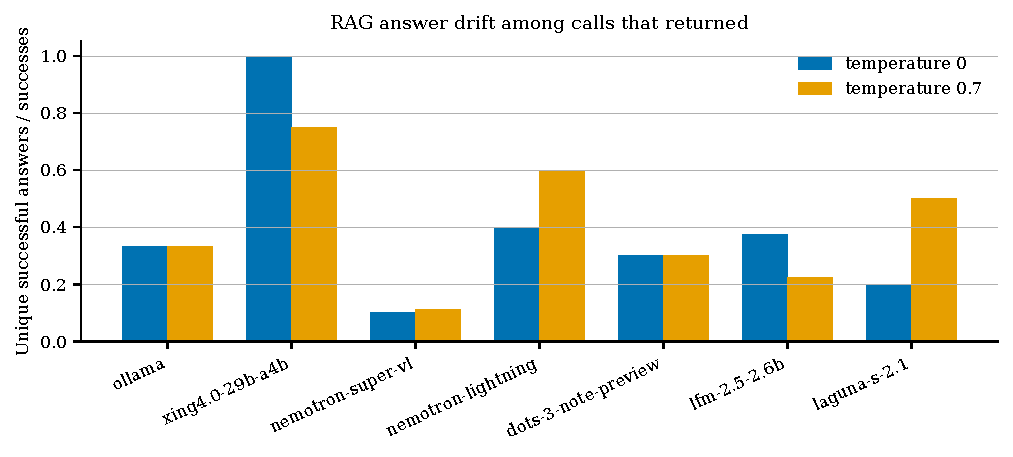
\includegraphics[width=\linewidth]{rw-drift.pdf}
\caption{Distinct successful RAG answers divided by the number of successful calls. Ollama used n=3. Hosted rows use the successes recorded for that model.}
\label{fig:rw-drift}
\end{figure}

\begin{figure}[t]
\centering
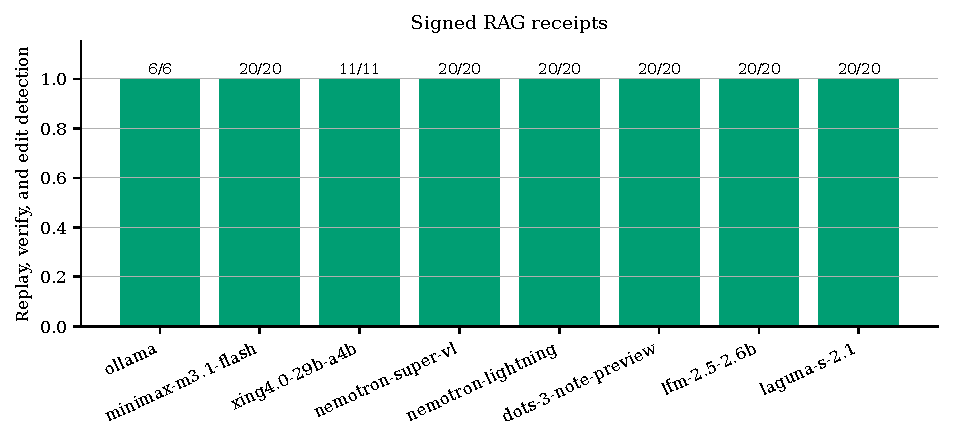
\includegraphics[width=0.9\linewidth]{rw-replay.pdf}
\caption{Receipts from calls that returned. Each counted receipt verified, replayed offline, matched the output hash, and detected a one-character edit. Rate-limited calls with no receipt are left out of the denominator.}
\label{fig:rw-replay}
\end{figure}

\begin{figure}[t]
\centering
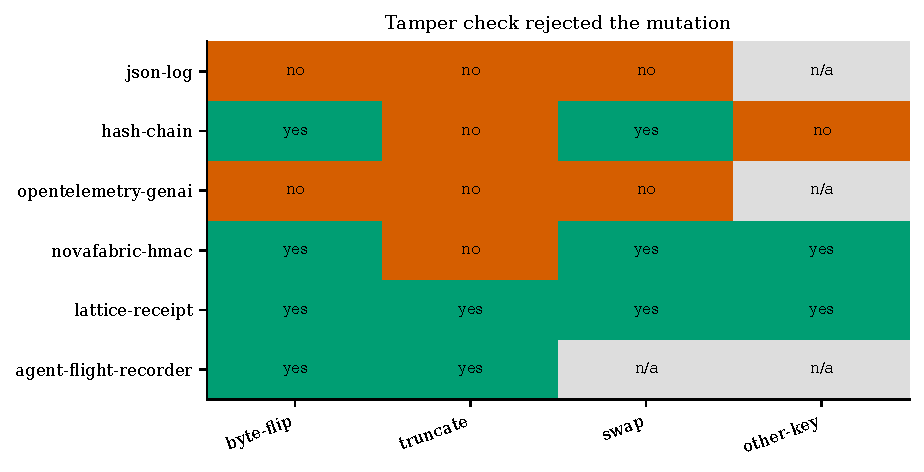
\includegraphics[width=\linewidth]{rw-tamper-heat.pdf}
\caption{Whether the system's own check rejects the mutation. Gray means that class was not applied. Truncating a hash chain leaves a valid prefix. A byte flip inside a JSON string, a dropped tail record, and a swapped response all remain valid JSON, so a parser does not catch them.}
\label{fig:rw-tamper-heat}
\end{figure}

\begin{figure}[t]
\centering
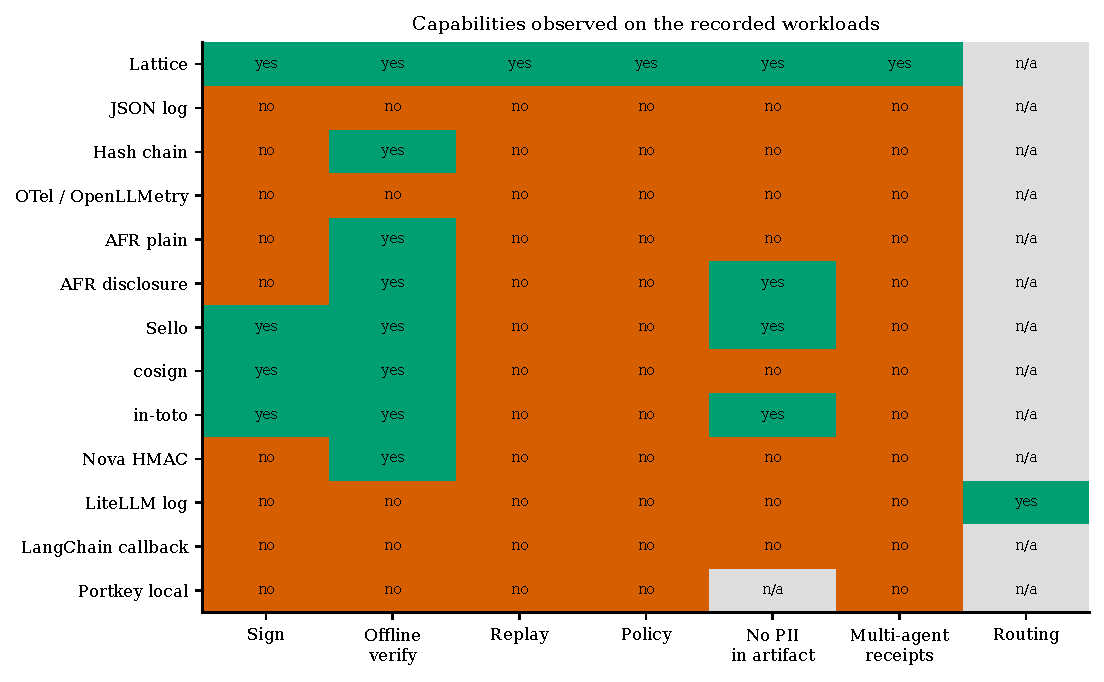
\includegraphics[width=\linewidth]{rw-capability.pdf}
\caption{Capabilities observed on these workloads. Gray is not measured here. LiteLLM routing is eight calls across two identical local deployments, which returned one route. Lattice routing is gray because each live call used one configured provider. Portkey's stored-log endpoint returned HTTP 500, so the PII cell is gray. LiteLLM's callback log stored the prompt text. The single-agent Lattice return carried no receipt; the crew return did.}
\label{fig:rw-capability}
\end{figure}

LiteLLM here is an in-process client, not a proxy process. Its router sent eight short prompts to two identical Ollama deployments and returned 1 distinct route across 8 calls. That is a weak determinism check. Helicone and Langfuse were not started.

\begin{table*}[t]
\centering
\caption{Local wrappers around Ollama. Marker detection scans the captured log or span. Portkey's log route failed, so that row does not show what a stored log would contain.}
\label{tab:rw-gateways}
\footnotesize
\resizebox{\textwidth}{!}{%
\begin{tabular}{@{}l l r r r l l l@{}}
\toprule
System & Status & n & p50 ms & Bytes & Markers in capture & Offline verify & Replay \\
\midrule
ollama-direct & measured & 5 & 1060.2 & --- & --- & --- & --- \\
litellm & measured & 5 & 3964.8 & 2408 & prompt stored & no & no \\
langchain-callback & measured & 5 & 1936.3 & 6893 & yes & no & no \\
openllmetry & measured & 3 & 1253.1 & 3346 & yes & no & no \\
portkey-gateway & measured & 5 & 6281.0 & 1953 & log unread & no & no \\
helicone & from docs, not measured & --- & --- & --- & --- & --- & --- \\
langfuse & from docs, not measured & --- & --- & --- & --- & --- & --- \\
\bottomrule
\end{tabular}}
\end{table*}

\begin{figure}[t]
\centering
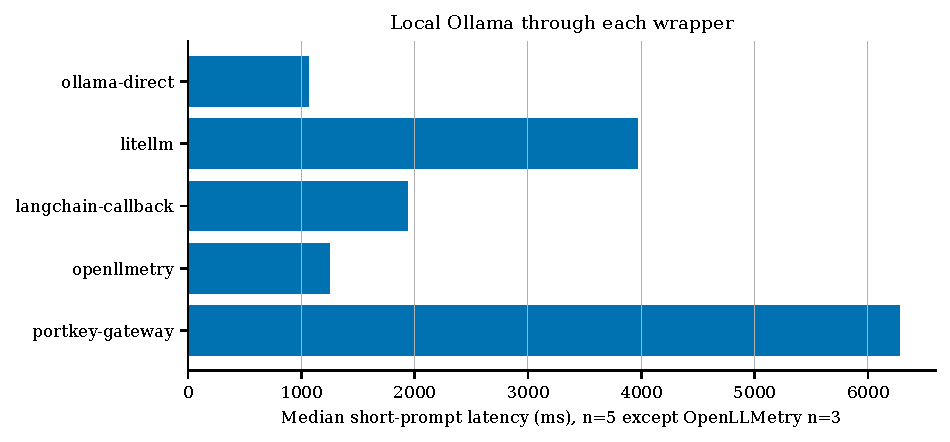
\includegraphics[width=0.86\linewidth]{rw-gateway-latency.pdf}
\caption{Median short-prompt latency through each local wrapper. OpenLLMetry used n=3. The other measured rows used n=5.}
\label{fig:rw-gateway-latency}
\end{figure}

